% EDIT HERE
% Enter team number below ??
\newcommand{\TeamNo}{31}
% Enter HW number below ??
\newcommand{\HWno}{01}
% 1st student information
\newcommand{\AuthorOneName}{Merve Nur Öztürk}
\newcommand{\AuthorOneID}{2311322}
% 2nd student information (leave empty if none)
\newcommand{\AuthorTwoName}{Atakan Süslü}
\newcommand{\AuthorTwoID}{2311371}
% 3rd student information (leavIDnumber1e empty if none)
\newcommand{\AuthorThreeName}{Betül Rana Kuran}
\newcommand{\AuthorThreeID}{2311173}
% END EDITING
% DO NOT MODIFY BELOW EXCEPT FOR ADDING PACKAGES #######
\documentclass[letterpaper,12pt]{article}
\usepackage{tabularx} % extra features for tabular environment
\usepackage{amsmath}  % improve math presentation
\usepackage{amssymb}
\usepackage{xcolor}
\usepackage{float}
\usepackage[export]{adjustbox}
\usepackage{graphicx} % takes care of graphic including machinery
\usepackage[margin=1in,letterpaper]{geometry} % decreases margins
\usepackage{cite} % takes care of citations
\usepackage{setspace}

\begin{document}
\begin{center}
AE 305, 2020-21 Fall \hfill \textbf{HW \HWno} \hfill \textbf{Team \TeamNo} \\
\noindent\rule{\textwidth}{0.4pt}
\begin{tabular}{p{0.33\textwidth} | p{0.33\textwidth} | p{0.33\textwidth} }
	\AuthorOneName&\AuthorTwoName&\AuthorThreeName\\
	\textit{\AuthorOneID}&\textit{\AuthorTwoID}&\textit{\AuthorThreeID}
\end{tabular}
\noindent\rule{\textwidth}{0.4pt}
\end{center}

%Report start

\section{Introduction}

It is useful to use numerical methods in order to solve differential equations when
the analytical solution is time consuming. In this homework, we are given an aircraft
which rolls on the ground and takes off some time later, and we are asked to find
the minimum time required for this aircraft to take off at different airport altitudes.
We know that the aircraft will take off when the lift force is higher than the weight of
the aircraft. Since the lift force is a function of velocity;

\begin{equation}
        L = C_L \cdot \frac{1}{2} \cdot \rho_{\infty} \cdot V_{\infty}^{2} \cdot S
\end{equation}

first we should calculate velocity which is described in a differential form for
this problem using the force balance equation in the horizontal direction:

\begin{equation}
        \frac{W}{g} \cdot \frac{dV}{dt} = T - D - \mu \cdot (W - L)
\end{equation}

where the lift and drag forces are initially zero. The next values of drag force is calculated
by this formula:

\begin{equation}
        D = C_D \cdot \frac{1}{2} \cdot \rho_{\infty} \cdot V_{\infty}^{2} \cdot S
\end{equation}

Therefore we are asked to use Euler's and RK2 methods so that we can approach the
solution with the help of numerical methods.


\section{Method}
Euler's method can be defined as the first order Taylor Series Expansion. In this method, the space between
the initial point of the independent variable and the desired next point is divided into discrete points. The 
difference between respective discrete points is named as step size, $\Delta x$. Then, a first order ordinary
differential equation at initial point, is calculated and treated as slope.
\begin{equation}
\frac{dy}{dx} \equiv y \prime \equiv f(x,y) \equiv SLOPE
\end{equation}
The slope is multiplied by the stepsize
and added to initial dependent variable. The result gave the next dependent variable.

\begin{center}
Next Value = Previous Value + Step Size $\times $ Slope
\end{center}
\begin{equation}
y(x + \Delta x ) = y(x) + \Delta x f(x,y)
\end{equation}
\begin{equation}
y_{i+1} = y_i + \Delta x f(x_i , y_i)
\label{eq:eul}
\end{equation}
This equation was repeated until the $x_i$ exceeded the desired independent point.

Second Order Runge-Kutta method has the similar equation form with Euler's method:
\begin{equation}
y_{i+1} = y_i + \Delta x \phi (x_i , y_i, \Delta x)
\label{eq:rk2}
\end{equation}
However, in second order RK method, $y\prime $ is not used as slope. In stead of $y\prime $, $\phi$ which is 
called increment function is used. $\phi$ is weighted slope function over the interval.
\begin{equation}
\phi = a_1k_1 + a_2k_2
\end{equation}
\begin{center}
$ \frac{dy}{dx} = f(x,y) $  

\doublespacing
$k_1 = f(x_i,y_i)$ 

\doublespacing
$k_2 = f(x_i+p_i\Delta x, y_i+p_i\Delta x k_1)$
\end{center}
where $p_i<1$  and
We chose $p_i = 2/3 $.
\begin{center}
$a_1+a_2 = 1$ 

\doublespacing
$a_2p_1 = \frac{1}{2}$
\end{center}
Therefore, $a_1=1/4$ and $a_2=3/4$ .
Trapezoidal integration rule is basic version of calculating area under a curve. It is based on
dividing the area under the curve $y(x)$ into small trapezoids. Then, areas of trapezoids which was equal to 
$\frac {1}{2}(V_i+V_{i+1})\Delta t $ is summed up:
\begin{equation}
\int_{0}^{N_p\Delta t} V(t) dt = \sum_{i=0}^{N_p-1} \frac{1}{2}(V_i+V_{i+1}) \Delta t 
\end{equation}

\newpage

\section{Results and Discussion}

\subsection{Calculation of velocity at sea level with Euler's Method }
\begin{figure}[ht]
\centering 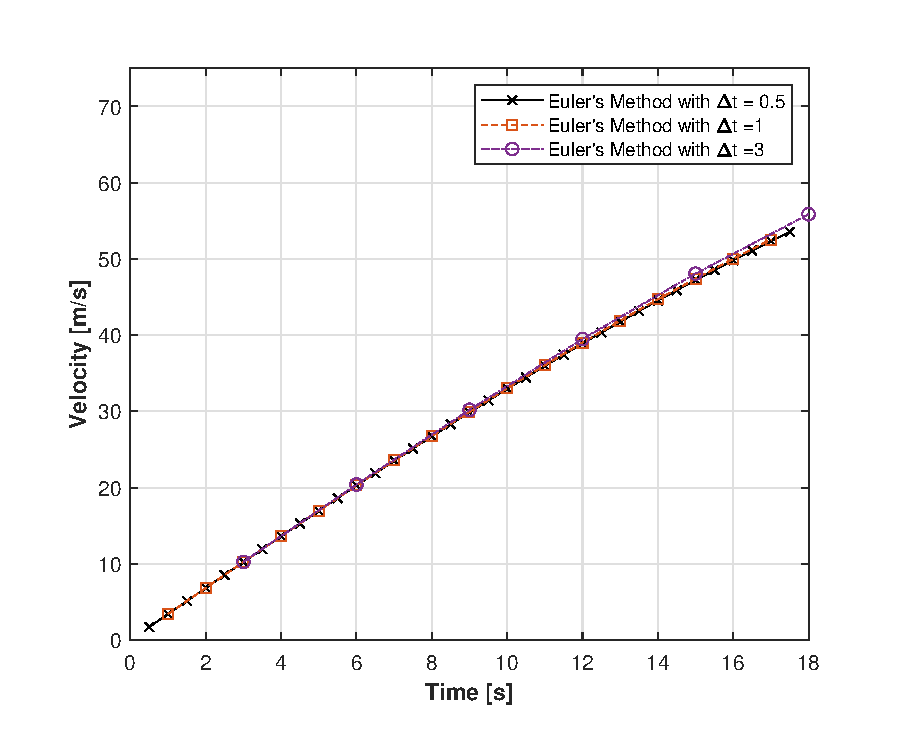
\includegraphics[max height=10cm]{graphs/question1.eps}
\caption{Calculation of velocity using Euler's Method with three different time steps at sea level.}
     \label{fig:q1}
\end{figure}

As can be seen in Figure \ref{fig:q1}, using different time steps gives different results.
Initially, results were approximately the same but as time progresses, margin of error increases.
This margin of error is different for each time step. When $ \Delta t = 3 $, error grows faster than
other step sizes.

\newpage
\begin{figure}[ht]
        \centering 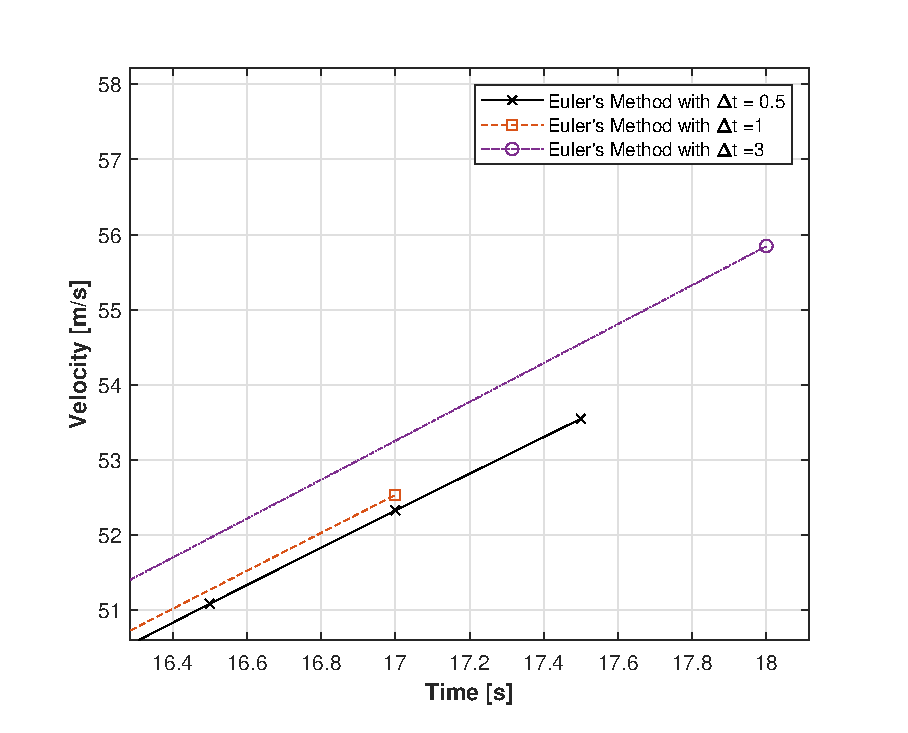
\includegraphics[max height=10cm]{graphs/question1_finaltime.eps}
        \caption{Detailed version of Figure \ref{fig:q1} focused on the endpoints.}
        \label{fig:q1_closer}
\end{figure}

 The effects of different time steps on result can be clearly seen in Figure \ref{fig:q1_closer}. If we want to obtain
 more precise result, we must decrease the step size.
\newpage
\subsection{Calculation of velocity at different altitudes with Euler's Method }
\begin{figure}[ht]
        \centering 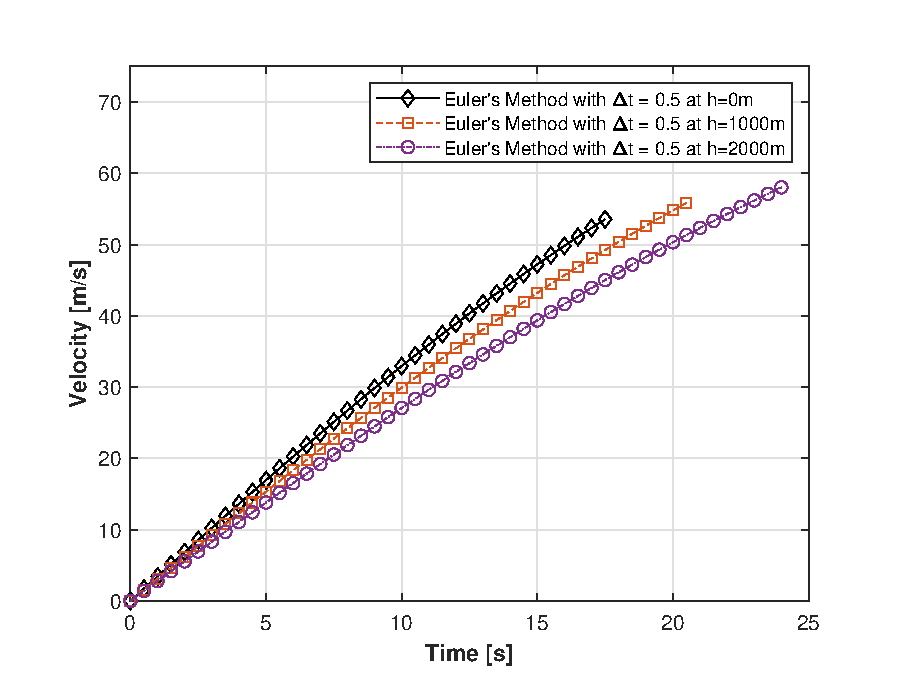
\includegraphics[max height=10cm]{graphs/altitude.eps}
        \caption{Calculated velocities at different altitudes using Euler's method with $\Delta t = 0.5$.}
        \label{fig:altitude}
\end{figure}

It can be obtained from Figure \ref{fig:altitude} that it takes longer to take off at higher altitudes. 
This is because as the altitude increases, air density decreases, which decreases the maximum available
thrust. In addition, lift and drag forces also decrease. Decrease in drag should normally decrease 
take off time while the decrease in thrust and lift does exactly the opposite. However, 
the effect of decrease in both lift and thrust overcomes the effect of drag. Therefore 
take off time increases in higher altitudes.

\subsection{Placeholder}

\section{Conclusion}

\end{document}